% Created 2011-11-19 sam. 18:27
\documentclass[11pt]{article}
\usepackage[utf8]{inputenc}
\usepackage[T1]{fontenc}
\usepackage{fixltx2e}
\usepackage{graphicx}
\usepackage{longtable}
\usepackage{float}
\usepackage{wrapfig}
\usepackage{soul}
\usepackage{textcomp}
\usepackage{marvosym}
\usepackage{wasysym}
\usepackage{latexsym}
\usepackage{amssymb}
\usepackage{hyperref}
\tolerance=1000
\providecommand{\alert}[1]{\textbf{#1}}

\title{Spécifications}
\author{Cherif Ibrahim, Quentin Loïc, Vilver Jean}
\date{21 Novembre 2011}

\begin{document}

\maketitle

\setcounter{tocdepth}{3}
\tableofcontents
\vspace*{1cm}

\section{Interprétation du sujet}
\label{sec-1}
\subsection{Compréhension}
\label{sec-1-1}
L'objectif est de concevoir un moteur de jeu d'échecs respectant fidèlement (note vers les règles de la FIDE) les règles de ce jeu, et capable d'acceuillir un certain nombre d'extensions futures.

Ce moteur doit tout d'abord contenir les fonctionnalités de bases du jeu d'échecs : une représentation du plateau du jeu, la position courante sur le plateau, les coups légaux pour un joueur à partir d'une position donnée et l'obtention d'un gagnant à la fin de la partie.
   
Il convient ensuite de réfléchir sur le rôle même d'une extension. Une ex tension au jeu d'échecs correspondrait-elle à une altération du jeu en lui-même, par exemple en ayant un plateau plus grand, ce qui n'est pas permis dans les règles de ce jeu. Ou en restant dans le cadre même du jeu, en offrant par exemple la possibilité de jouer à la pendule.
   
On choisira de considérer que toutes nouvelles fonctionnalités à la version de base, respectant les règles ou non, seront considérées comme des extensions, afin de laisser le plus de liberté à l'évolution du système dans le temps. 
En effet, des extensions mettront à l'épreuve l'architecture initiale, donc plus la liberté d'évolution sera grande, plus les chances de pouvoir intégrer ses extensions, sans modification du code, sera grande.
\subsection{Problèmes techniques}
\label{sec-1-2}
\subsubsection{Le protocole CECP}
\label{sec-1-2-1}
On comprend que le protocole CECP permet la communication entre le moteur de jeu et l'interface utilisateur. La diffulté est de comprendre où il intervient précisément dans moteur du jeu.

Avec l'utilisation du modèle MVC, l'emplacement du protocole dans le système s'éclairci. Lorsque l'interface envoie une requête, elle l'envoie vers le contrôleur, qui notifie ensuite le modèle de cette requête. Ensuite, le modèle envoie les actions à effectuer à toutes les vues. 

Il convient donc de positionner le protocole entre le contrôleur et la vue, puis entre le modèle et les vues. Le protocole jouera donc le rôle de traducteur entre ces différents éléments.
\newpage
\section{Concepts}
\label{sec-2}
\subsection{Problèmes conceptuels}
\label{sec-2-1}
À travers l'étude du sujet, les questions suivantes se sont posées: Comment rendre le moteur le plus général et modulaire possible ? Comment représenter la versatilité des pièces, et modéliser la promotion du pion ? Comment prendre en compte la possibilité d'optimiser l'occupation mémoire du système ? Si l'on désire pouvoir consulter un historique de la partie, comment peut-on l'écrire ? À partir de la décision d'utiliser un modèle MVC pour le projet, quel ensemble de constituants représentera le Modèle, les Vues et le Contrôleur ?

\subsection{Solutions}
\label{sec-2-2}
La plupart de ces questions trouvent une réponse avec l'utilisation de Design Patterns. En effet, l'utilisation du patron Strategy permet de rendre le mouvement de chaque pièce dynamiquement modifiable, ce qui facilite la gestion des promotions des pions. De la même façon, l'occupation mémoire peut être optimisée si le besoin se présente grâce au patron Flyweight (Poid mouche). Afin de combiner ces deux composants pour obtenir un système de gestion de pièces dépendant des exigences de l'utilisateur, l'utilisation du patron Factory (Usine) s'est imposée. Pour la même raison, ce patron sera utilisé dans la représentation du plateau, afin de pouvoir gérer l'éventualité du support de jeux de plateau différents du jeu d'échecs, avec par exemple plus de cases, plus de joueurs, ou plus de dimensions. Pour ajouter au système la gestion d'un historique, le patron Memento a semblé la meilleure réponse, puisque destiné à ce genre de situations.

En suivant ces réflexions, l'ensemble constitué du plateau et des pièces représentera le Modèle dans notre système, les Vues seront les clients tels que XBoard, et le rôle du Contrôleur est rempli par [INSERER ICI L'ENSEMBLE CORRESPONDANT].

Les patrons de conceptions décrits ici seront décrits plus en détails par la suite.
\newpage
\section{Description de l’architecture}
\label{sec-3}
\subsection{Cas d'utilisation}
\label{sec-3-1}
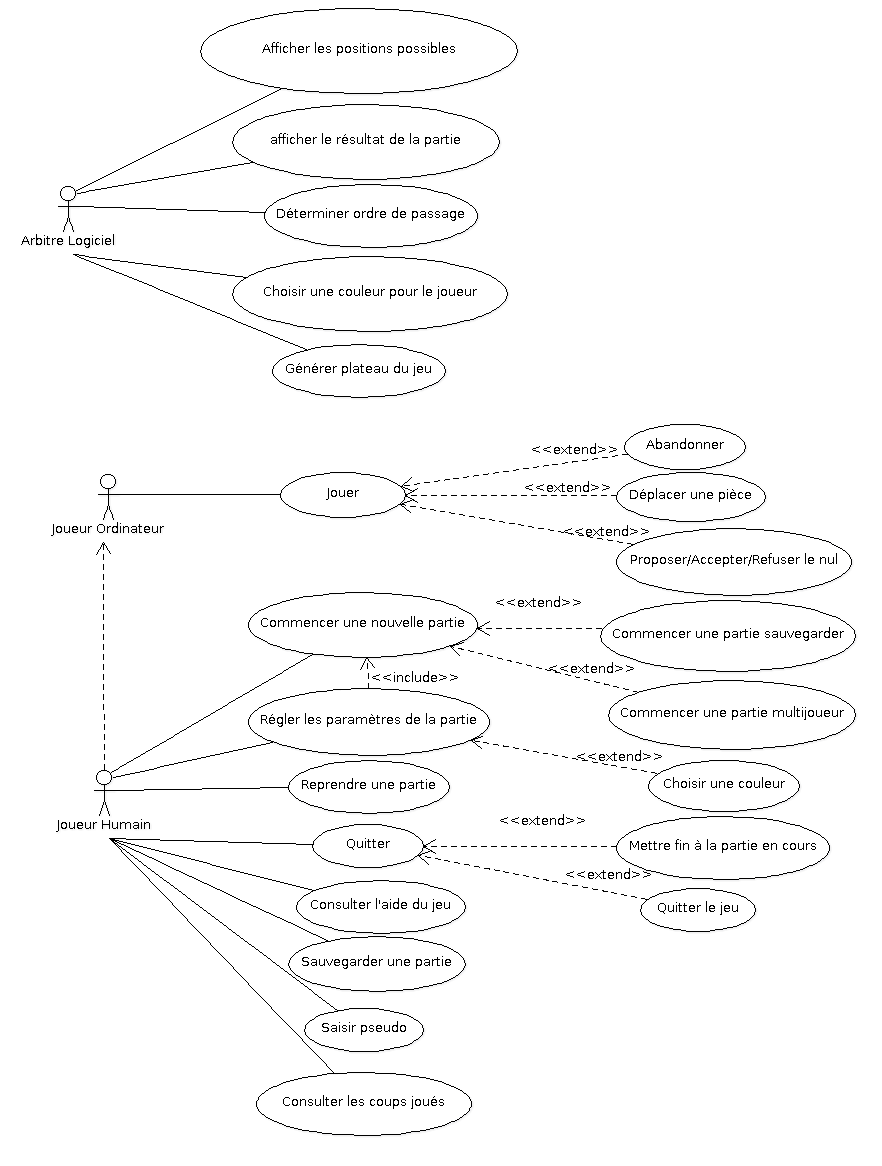
\includegraphics[width=0.9\textwidth]{Diagrammedecasdutilisation.png}

\subsection{Diagramme de classes}
\label{sec-3-2}
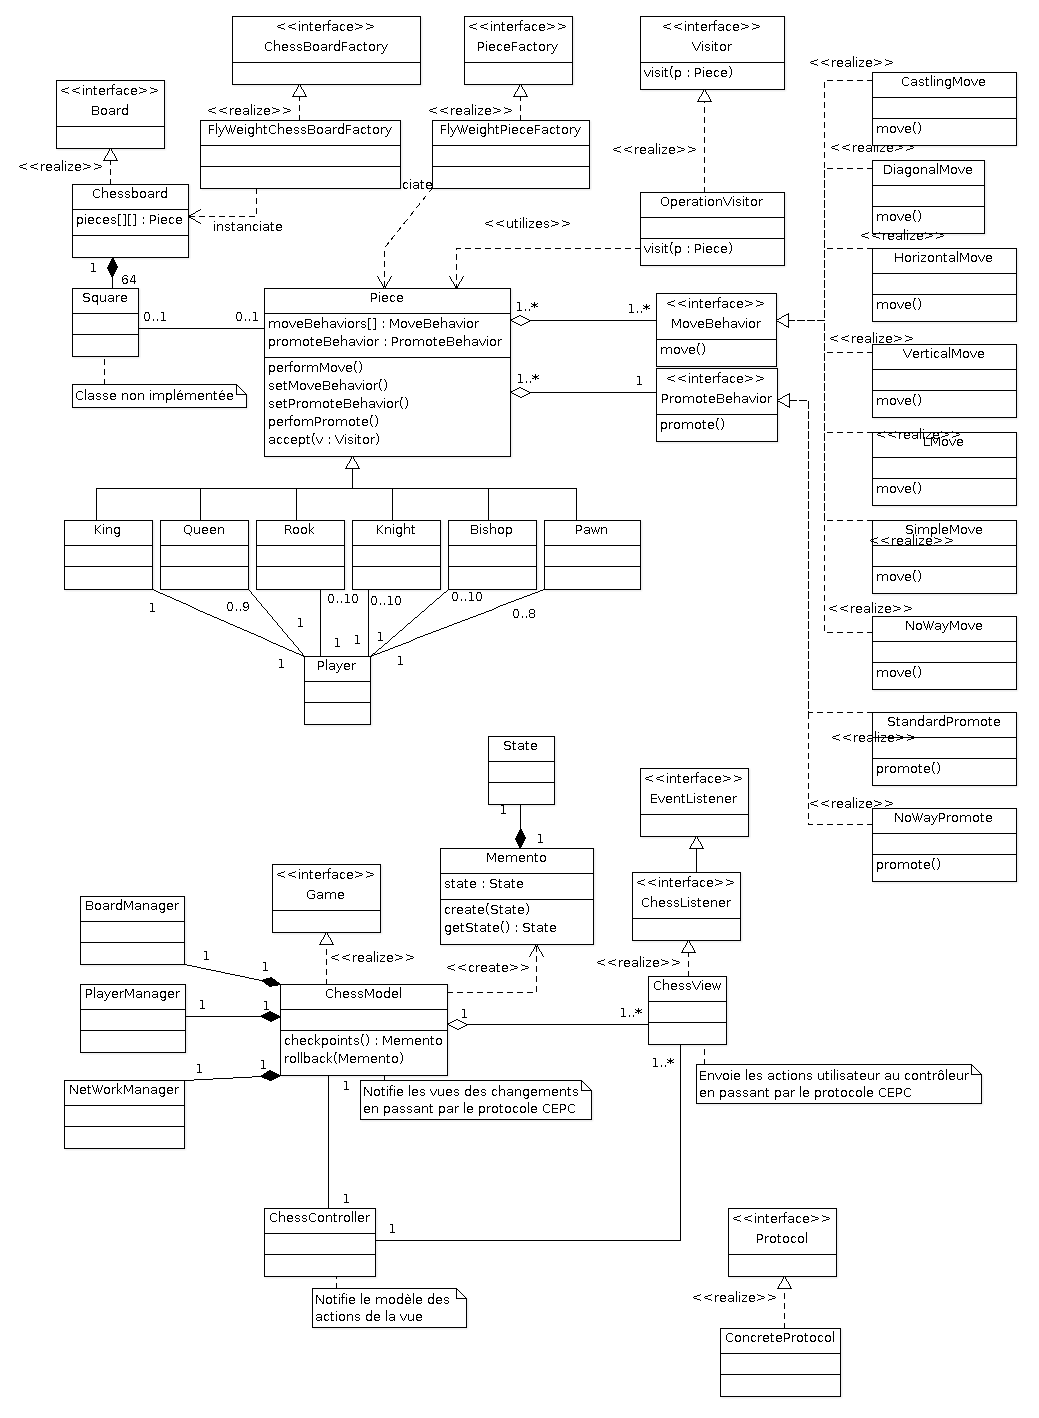
\includegraphics[width=0.9\textwidth]{Diagrammedeclasses.png}

\subsection{Patrons de conception utilisés}
\label{sec-3-3}
\subsubsection{Memento}
\label{sec-3-3-1}
Le patron de conception Memento est d'abord destiné à stocker l'état d'un composant, afin de pouvoir ensuite restaurer cet état. Il est très souvent utilisé lorsqu'on désire inclure une fonctionnalité \emph{``Undo''} dans un logiciel. Dans notre cas, une fois un coup joué, il n'est pas possible de revenir en arrière, cependant, la conservation de l'état du plateau et des pièces pemret d'écrire un historique de la partie, utile pour des joueurs stratèges qui désireraient étudier le déroulement de leur parties, pour y découvrir les raisons de leur défait ou victoire.
\subsubsection{Factory}
\label{sec-3-3-2}
Le patron de conception Factory permet de séparer l'implémentation concrète d'un composant de sa spécification: ainsi, il est possible de changer d'implémentation selon le besoin, par exemple, si un grand nombre de pièces est nécessaire, ou que l'on désire minimiser l'impact en mémoire du système, on pourra appeller une version implémentant le patron Flyweight pour notre usine de pièces.
\subsubsection{Flyweight}
\label{sec-3-3-3}
Le patron Flyweight permet d'économiser de la mémoire en représentant de l'information sans une instanciation automatique. On peut par exemple, représenter tous les pions en ne créant en réalité qu'un seul pion et en sauvegardant les différences entre les pions.
\subsubsection{Strategy}
\label{sec-3-3-4}
Ce patron permet la modification à un seul endroit d'un comportement si ce comportement est utilisé par plusieurs pièces ainsi que la réutilisation d'un comportement pour une nouvelle pièce.
\subsubsection{MVC}
\label{sec-3-3-5}
C'est un patron d'architecture et une méthode de conception qui organise l'Interface Homme Machine. Il se divise en trois parties: les Vues, le Modèle et le Contrôleur.
\paragraph{Vues} : Il n'est pas demandé de développer une interface graphique pour jouer aux échecs. Cependant, il est nécessaire d'implémenter un sous-ensemble du protocole CECB, afin d'utiliser par la suite une interface externe implémentant ce protocole.
En général, les vues sont les interfaces avec lesquelles l'utilisateur interagit.
\paragraph{Modèle} : Il représente dans l'architecture MVC le comportement de l'application. En effet, il prend en charge la manipulation et la gestion des données. Dans notre cas il assure la création de la table, l'initialisation du jeu, et tous les changements effectués sur les pièces et le jeu en général (BoardManager). Il assure aussi le déroulement des parties sur le réseau (NetworkManager), et tout ce qui concerne la gestion de joueurs (PlayerManager). Notons que tout ce qui se déroule au niveau du modèle est transféré aux vues en passant par le protocole CECP.
\paragraph{Contrôleur} : Il a comme tâche de transmettre les modifications et d'assurer la synchronisation. Il prend en charge la réception des actions effectuées coté vues par l'utilisateur (où la transmission est assurée par le protocole CECP) et la notification au modèle de ces actions.
\newpage
\section{Extensions envisagées}
\label{sec-4}
\subsection{Ajout de nouvelles pièces}
\label{sec-4-1}
Grâce à l'abstraction de la notion de pièce du jeu via la classe abstraite \emph{Piece}, et à l'utilisation des comportements à travers le patron Strategy, il est possible d'ajouter ou de modifier le comportement des pièces du jeu. Ainsi, il est envisageable de réutiliser ce moteur pour implémenter un moteur de jeu de Dames plutôt de que d'échecs, à l'aide d'une nouvelle classe dédiée de pion et d'une classe gérant son mouvement et sa promotion.
\subsection{Changement de capacité de mouvement d'une pièce}
\label{sec-4-2}
L'utilisation du patron Strategy permet de séparer la façon dont les pièces peuvent se déplacer sur le plateau. Ainsi, il est aussi possible d'ajouter des comportements aux pièces, et donc de créer de nouvelles pièces, en combinant de façon différente les comportements déjà existant, ou en créant de nouveaux comportements pour les pièces déjà existantes, ou combinaison de ces deux possibilités. Notons que ceci permet aussi de modifier le comportement des pièces dynamiquement.
\subsection{Changement de capacité de promotion}
\label{sec-4-3}
De la même façon que le patron Strategy permet d'autoriser l'extension par ajout de comportement de mouvement d'une pièce, il permet ici d'autoriser l'extension par changement de la façon dont les pièces peuvent être promues (dans le cas du jeu d'échecs, de Pion à Dame ou Tour, par exemple).
\subsection{Sauvegarde l'état d'une partie}
\label{sec-4-4}
La possibilité de sauvegarder une partie en cours est laissée comme perspective future d'extension du système. Ceci est rendu possible par l'utilisation du patron Memento, qui stocke l'état du plateau régulièrement.
\subsection{Extension non envisagées}
\label{sec-4-5}
Afin de permettre l'extension \emph{a posteriori} de notre système, de façons non imaginées par ses développeurs initiaux, le patron de conception Visitor (Visiteur) a été ajouté à la modélisation, pour qu'un contributeur externe n'ayant pas forcément accès à la source puisse ajouter ses fonctionnalités librement.

\end{document}
